\documentclass[conference,9pt]{IEEEtran}

\usepackage[utf8]{inputenc}
\usepackage{gensymb}
\usepackage[english]{babel}
\usepackage{graphicx}
\usepackage{amsmath,amssymb}
\usepackage{hyperref}
\usepackage{booktabs}
\usepackage{setspace}
\usepackage{enumerate}
\usepackage{listings}
%\usepackage{geometry}
\usepackage{float}


\usepackage{listings}
\usepackage{xcolor}

% Define a style for Python code
\lstset{
    language=Python,
    basicstyle=\ttfamily\small,
    keywordstyle=\color{blue},
    commentstyle=\color{gray},
    stringstyle=\color{red},
    showstringspaces=false,
    numbers=left,
    numberstyle=\tiny\color{gray},
    frame=single,
    breaklines=true,
    tabsize=4,
    captionpos=b,
    morekeywords={nn, self, super},
}

%\geometry{margin=1in}

\title{Global Weather Pattern Prediction for Disaster Preparedness}
\author{\IEEEauthorblockN{Jonas Thalmeier, Ana Martinez}}
\date{\today}

\begin{document}

\maketitle


\section{Introduction}
Effective identification and prediction of heatwaves are critical for public health, agriculture, and energy management. To accomplish this, a dataset containing atmospheric measurements was downloaded from the Copernicus Climate Data Store (CDS)\footnote{\url{https://cds.climate.copernicus.eu/}}. The dataset in use is ERA5, which provides hourly atmospheric reanalysis data with a high temporal and spatial resolution. As part of this project, steps were taken to extract spatially and temporally restricted subsets of ERA5 data and to apply percentile-based definitions of heatwaves.

This report details the intermediate steps undertaken: data acquisition, preprocessing, feature labeling, and initial approaches to building machine learning models for predicting future heat events. The approach followed best practices in data handling and model preparation, ensuring that the methodology can be refined and improved in subsequent phases.

\section{Data Acquisition and Preprocessing}

\subsection{Dataset Selection and Constraints}
\label{sec:DS}
The ERA5 dataset was accessed through the Climate Data Store after creating an account on the platform. Due to storage and download constraints, the spatiotemporal coverage had to be limited. Therefore, only data covering the territory of Spain were selected. Furthermore, since full hourly coverage would be voluminous, only two daily time points (00:00 and 12:00 UTC) were chosen.\\
For the first experiments a dataset with the following features was generated:
\begin{itemize}
    \item 2m temperature (t2m)
    \item 2m dewpoint temperature (d2m)
    \item Mean sea level pressure (msl)
    \item Total cloud cover (tcc)
    \item Volumetric soil water layer 1 (swvl1)
    \item 10m u-component of wind (u10)
    \item 10m v-component of wind (v10)
\end{itemize}
The dataset encompassed locations from 36\degree south to 44\degree north and 10\degree west to 4\degree east with a spatial grid width of 1\degree as well as all months of the year, with the intention of capturing a wide range of meteorological conditions. It was later observed that including all months, even those unlikely to produce heatwaves, was not the most efficient approach. Therefore a new dataset was generated. It only includes the month April to September. Since less days per year are included in the dataset, it was possible to lower the spatial resolution to a grid width of 0.25\degree. Furthermore the following features were added:
\begin{itemize}
    \item Surface Pressure (sp)
    \item Skin Temperature (skt)
    \item Boundary Layer Height (blh)
    \item Land-Sea Mask (lsm)
    \item Total Column Water Vapor (tcwv)
\end{itemize}

\subsection{Temporal and Spatial Restructuring}
After downloading the data in GRIB format, standard Python libraries such as \texttt{xarray} and \texttt{pygrib} were used for reading and handling the dataset. The data were initially organized by time and location. To simplify the learning task, measurements recorded at 00:00 and 12:00 for the same day and location were combined, presenting them as features side-by-side within a single row. This reformatting streamlined the input for the machine learning model, ensuring that each daily record included both early morning and midday conditions.

\section{Definition of Hot Days and Heatwaves}
\label{heatDef}
The Spanish meteorological service defines a heatwave as a sequence of at least three consecutive days during which the maximum daily temperature at a given location exceeds the 95th percentile of the daily maximum temperature distribution for July and August at that location. To implement this criterion, the temperatures at 12:00 for July and August were extracted from the ERA5 dataset. The 95th percentile threshold was then computed for each grid point (latitude-longitude pair).

Subsequently, any day whose 12:00 temperature exceeded the computed local 95th percentile threshold was labeled as a ``hot day.'' Rolling computations were carried out to identify sequences of three or more consecutive hot days (i.e., potential heatwave events). These computations confirmed the occurrence of multi-day hot periods in certain locations and provided an initial assessment of the frequency and distribution of heatwave events.

\section{Labeling and Feature Engineering}
To train a predictive model, labels indicating whether a heatwave would occur in the near future were needed. For each 30-day period (rolling window of consecutive days), a binary label was assigned: 1 if at least 3 hot days would occur in the following 7 days, and 0 otherwise. This labeling strategy provided a supervised learning setup, enabling the prediction of imminent heatwave conditions based on recent weather patterns. At this stage, a challenge arose: only about 2.09\% of the labels were positive (indicating a future heatwave), resulting in a highly imbalanced dataset. 

To facilitate machine learning, the data from all consecutive 30-day periods were stacked so that each record included the full sequence of daily measurements for those 30 days. However, this approach constrained the model to utilize data from a single location exclusively for forecasting that specific location. While this is not the standard approach for weather prediction, it was adopted to simplify data processing to a manageable level. Additionally, the project aimed to evaluate how accurately weather could be predicted without incorporating data from surrounding regions.

To address memory overflow issues that arose during data processing, a chunk-based approach was implemented to save intermediate results to disk. Instead of retaining the entire dataset in memory, the data for each year was processed incrementally. This involved extracting rolling features and aligning them with the corresponding labels for each year separately. The features and labels were then flattened and concatenated with additional attributes, such as latitude, longitude, and percentile thresholds, before being saved as PyTorch tensors to disk. This strategy enabled the handling of large datasets by reducing the memory footprint and allowed for efficient data loading during training, as individual yearly chunks could be accessed and processed independently without loading the entire dataset into memory.

\section{Preliminary Modeling Approaches}
Initial attempts to predict heatwaves involved testing several machine learning models:
\begin{enumerate}[1.]
    \item A simple neural network (NN) with fully connected layers was trained on the transformed dataset.
    \item A deeper neural network architecture, employing additional layers and dropout, was also tested.
    \item A random forest classifier
    \item A eXtreme Gradient Boosting classifier
    \item A logistic regression model from torch
    \item A logistic regression model from sklearn
\end{enumerate}

\subsection{Neural Networks}
The initial trials were conducted using neural networks due to their versatility and ability to model complex relationships in data. Given their wide applicability across various domains, they were anticipated to deliver acceptable initial results for this task. For these trials, the initial smaller dataset was used. The first network architecture is shown below:
\begin{lstlisting}
class HotDayPredictor(nn.Module):
    def __init__(self, input_size):
        super(HotDayPredictor, self).__init__()
        self.fc = nn.Sequential(
            nn.Linear(input_size, 128),
            nn.ReLU(),
            nn.Linear(128, 64),
            nn.ReLU(),
            nn.Linear(64, 1),
            nn.Sigmoid())
\end{lstlisting}
Normalization was applied to the inputs using the global mean and standard deviation calculated from the training set. Despite these steps, the results were disappointing. The training loss decreased, but the validation loss stagnated or increased, indicating significant overfitting. As depicted in Figure \ref{fig:baseline}, the loss for the validation set was much higher than that of the training set.
\begin{figure}[!t]
    \centering
    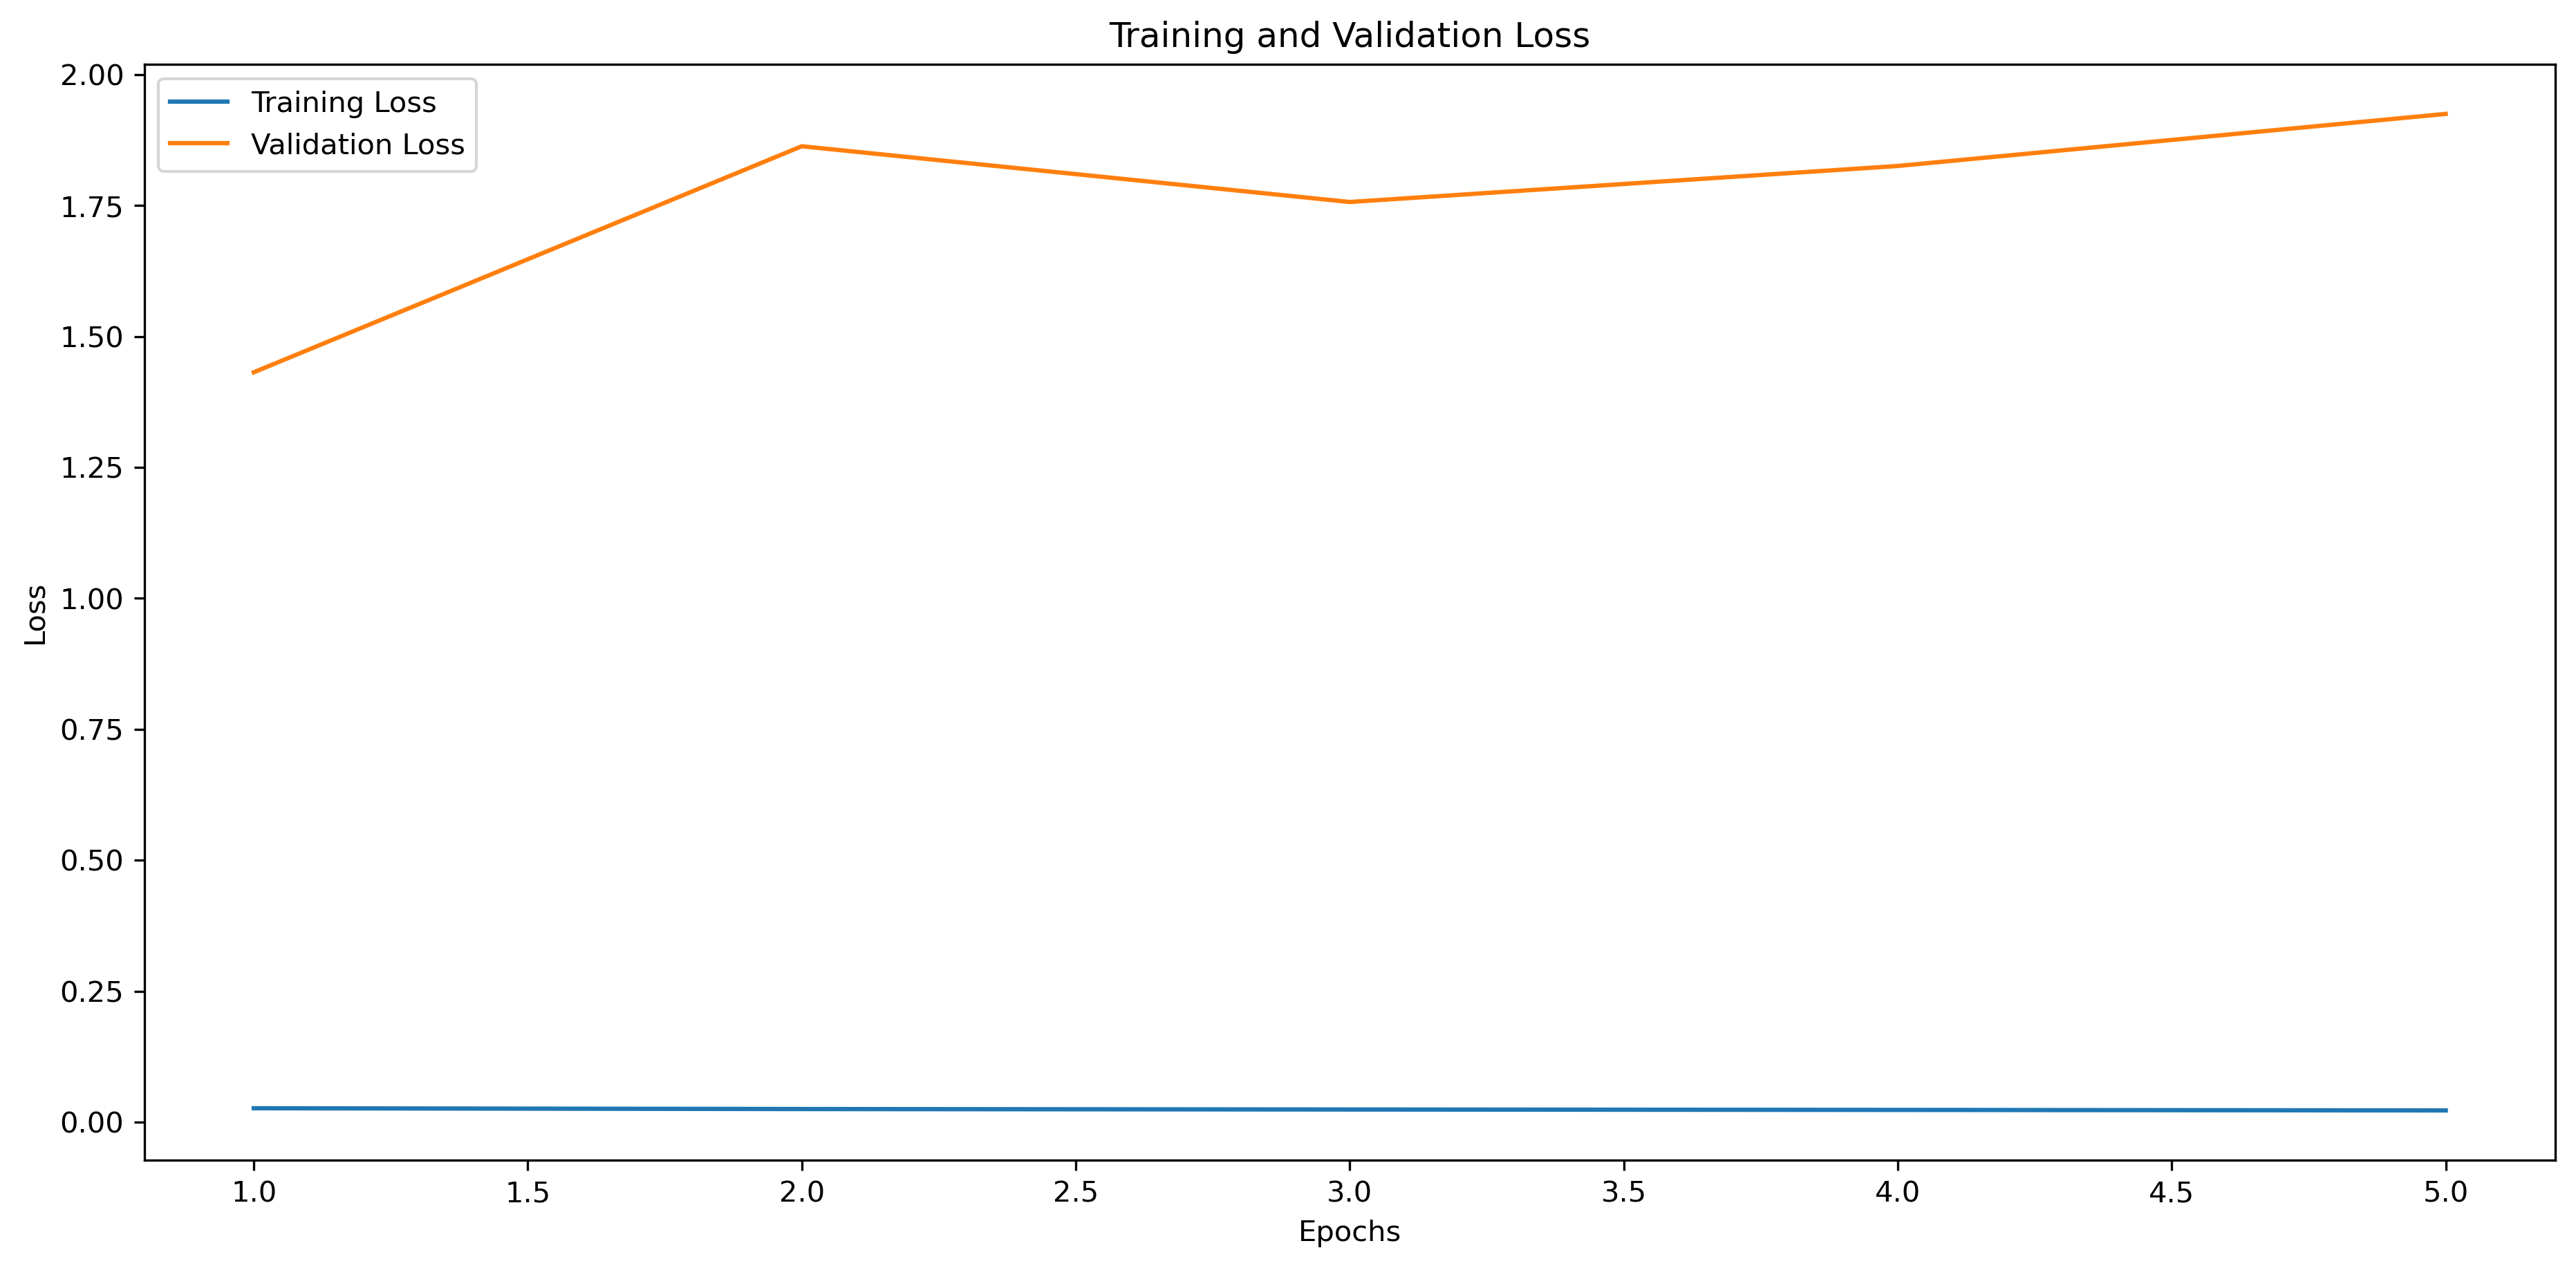
\includegraphics[width=\columnwidth]{../training_validation_loss_baseline.png}
    \caption{Evolution of training and validation loss}
    \label{fig:baseline}
\end{figure}
To address the overfitting, several iterations were undertaken to improve the network's generalization ability:
\paragraph{Iteration 1: Adding Dropouts and Weighted Loss}
Dropout layers were introduced to the architecture to mitigate overfitting by preventing co-adaptation of neurons. The modified architecture included dropout rates of 30\%:
\begin{lstlisting}
self.fc = nn.Sequential(
    nn.Linear(input_size, 128),
    nn.ReLU(),
    nn.Dropout(0.3),  # Add dropout of rate 30%
    nn.Linear(128, 64),
    nn.ReLU(),
    nn.Dropout(0.3),  # Add dropout
    nn.Linear(64, 1))
\end{lstlisting}
Additionally, a weighted loss function was implemented to address class imbalance:
\begin{lstlisting}
global_pos_weight = (global_total_count - global_positive_count) / global_positive_count
loss_fn = nn.BCEWithLogitsLoss(pos_weight=torch.tensor(global_pos_weight, dtype=torch.float32))
\end{lstlisting}
The learning rate was also reduced by a factor of 10 (to 0.0001). Despite these changes, overfitting persisted:
\begin{center}
    \begin{tabular}{c|c}
        Training Loss & Validation Loss \\ 
        \hline 
        0.311259 & 20.156125 \\
    \end{tabular}
\end{center}
\paragraph{Iteration 2: Adding Geospatial Features}
Longitude, latitude, and the 95th percentile temperature were added as additional features to each record. While this increased the dimensionality of the data, overfitting remained an issue, with a continued large discrepancy between training and validation loss. Validation loss increased further, indicating no improvement:
\begin{center}
    \begin{tabular}{c|c}
        Training Loss & Validation Loss \\ 
        \hline 
        0.299057 & 24.856614 \\
    \end{tabular}
\end{center}
\paragraph{Iteration 3: Expanded Dataset and Temporal Filtering}
An expanded dataset was generated, including additional variables as described in section \ref{sec:DS}. Despite these enhancements, overfitting persisted:
\begin{center}
    \begin{tabular}{c|c}
        Training Loss & Validation Loss \\ 
        \hline 
        0.282310 & 22.825080 \\
    \end{tabular}
\end{center}
The dataset was limited to land masses using the Land-Sea Mask (lsm) feature included in the dataset. This approach was based on the expectation that weather behavior differs significantly between land and sea, and thus predictions might be easier when focusing exclusively on land areas. However, this restriction significantly reduced the data diversity, leading to an even stronger overfitting effect:
\begin{center}
    \begin{tabular}{c|c}
        Training Loss & Validation Loss \\ 
        \hline 
        0.1613860 & 31.200668 \\
    \end{tabular}
\end{center}
\paragraph{Evaluation Metrics}
The following evaluation metrics illustrate the poor generalization of the model:
\begin{center}
    \begin{tabular}{c|c|c|c}
        Accuracy & Precision & Recall & F1 Score \\ 
        \hline 
        0.8951 & 0.1166 &  0.0436 & 0.0635\\
    \end{tabular}
\end{center}
Despite various attempts to mitigate overfitting, the neural network failed to generalize effectively, necessitating a shift to alternative modeling approaches. As shown in Figure \ref{fig:It3}, the model's performance remains unsatisfactory after all iterations. The training loss continues to decrease steadily, while the validation loss either stagnates or increases, indicating persistent overfitting and the inability of the model to generalize to unseen data.
\begin{figure}[!t]
    \centering
    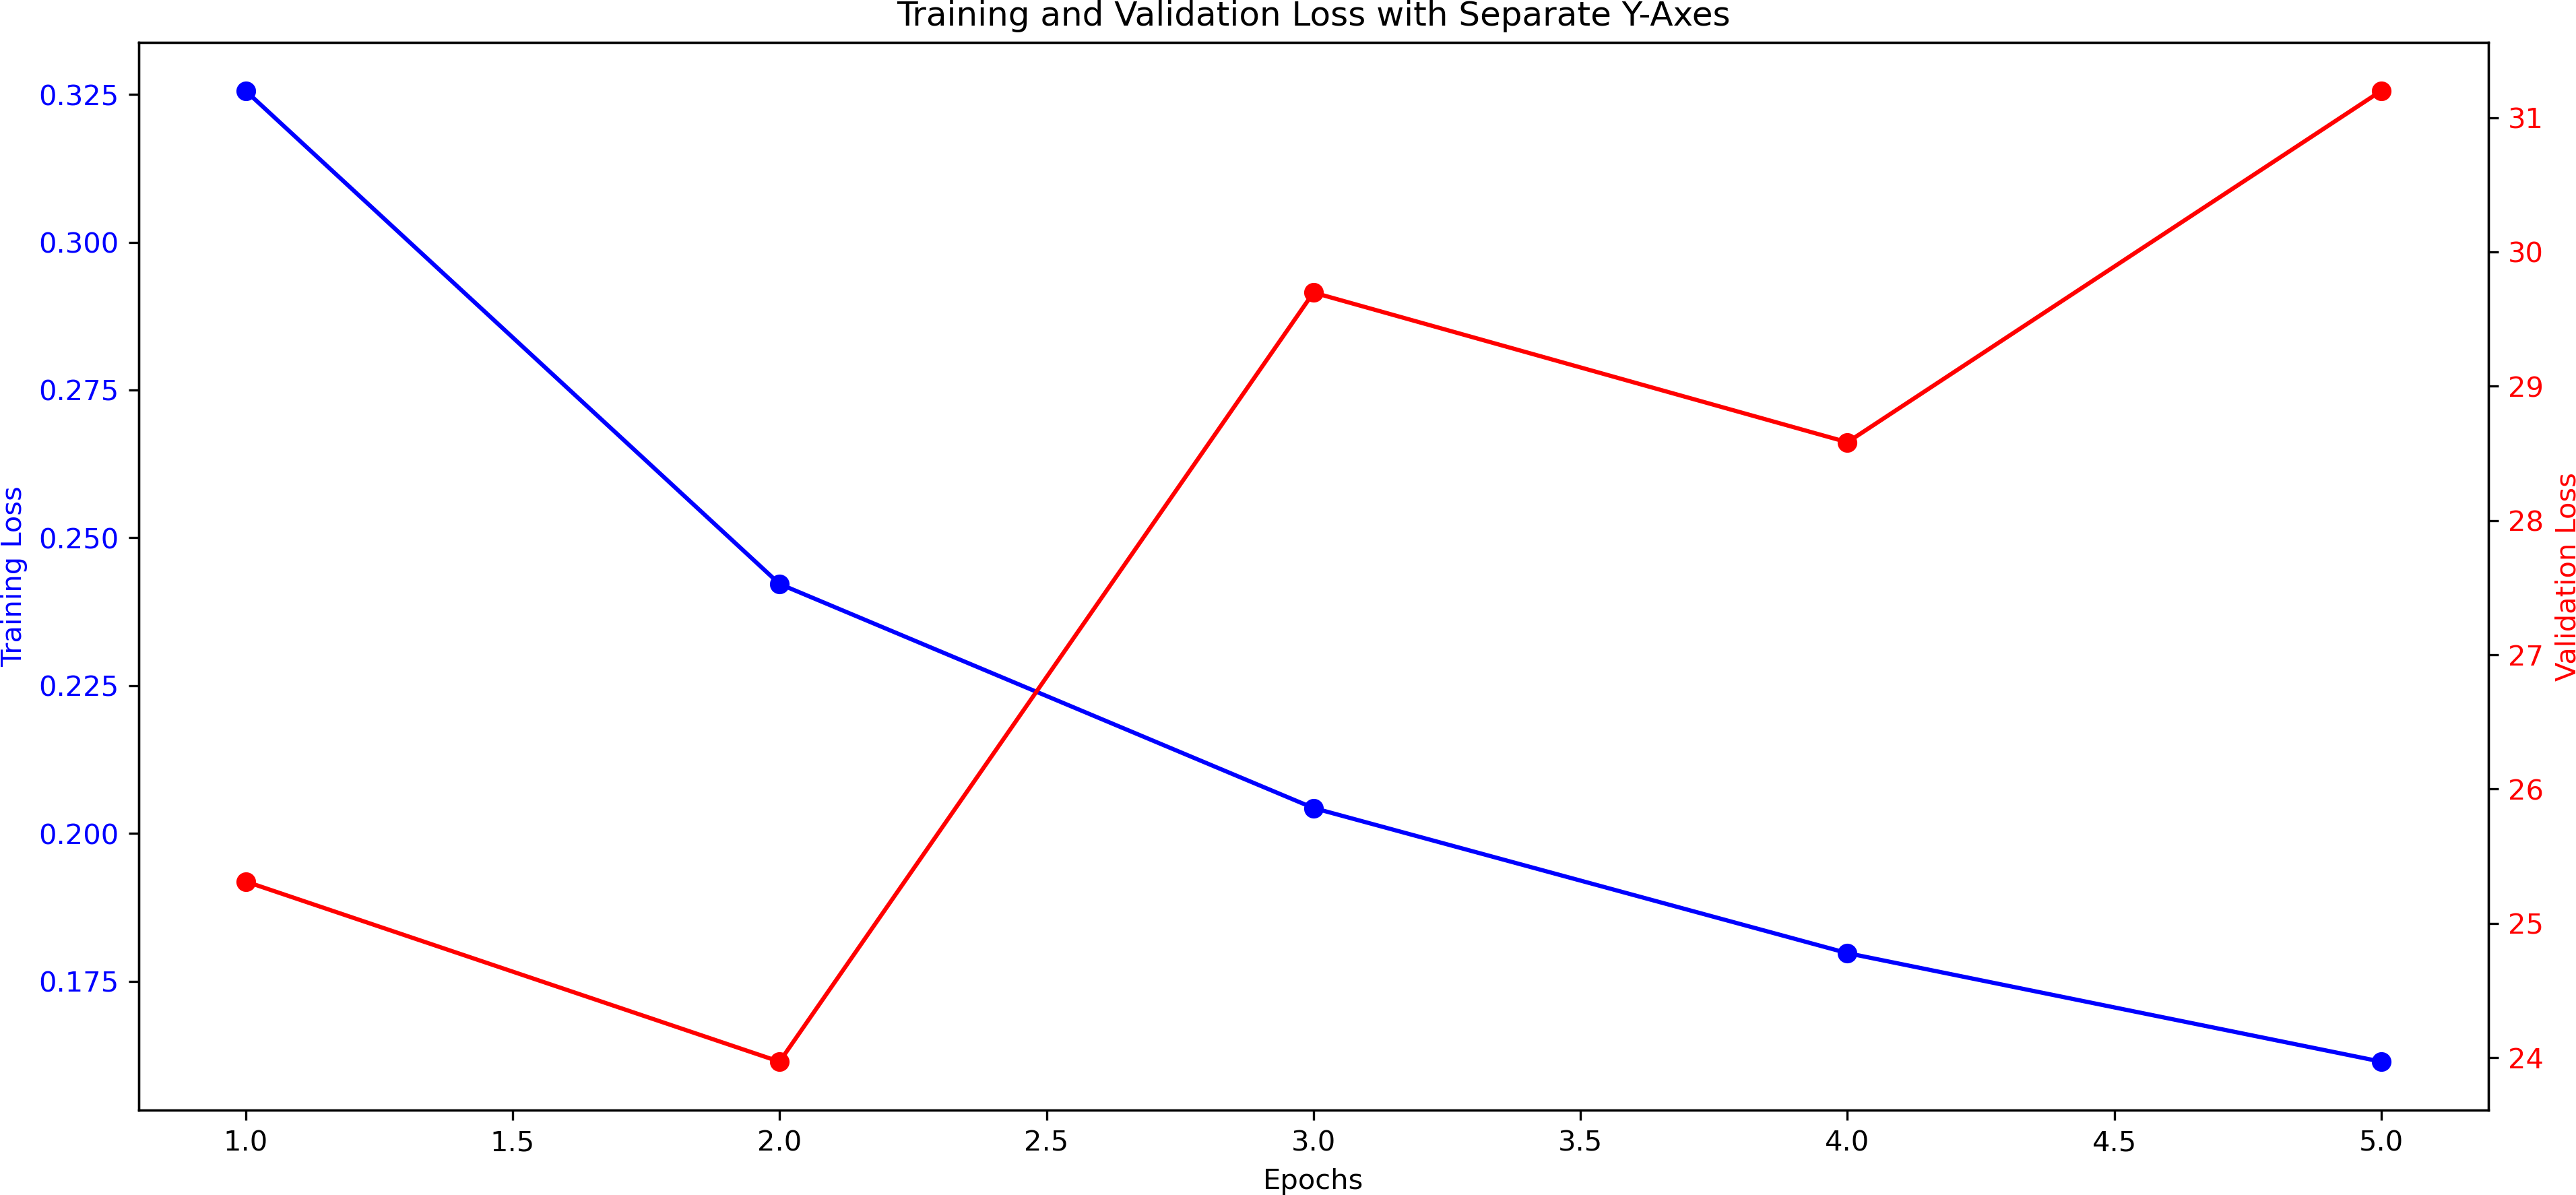
\includegraphics[width=\columnwidth]{../training_validation_loss_Iteration3.png}
    \caption{Evolution of training and validation loss after 3rd Iteration of NN model}
    \label{fig:It3}
\end{figure}

\subsection{Random Forest}
Random forests were employed due to their robustness and ability to handle high-dimensional data without extensive preprocessing. They also naturally account for feature importance, which can provide insights into the data. For this experiment, the entire training set was used, and hyperparameters such as the number of estimators and maximum tree depth were tuned.
The model was trained using the following parameters:
\begin{lstlisting}
rf_model = RandomForestClassifier(
	n_estimators=500,
	max_depth=20,
	random_state=42,
	class_weight="balanced")
\end{lstlisting}
Data preprocessing included normalizing the features using the global mean and standard deviation calculated from the training set. The random forest achieved the following results on the test set:
\begin{center}
    \begin{tabular}{c|c|c|c}
        Accuracy & Precision & Recall & F1 Score \\ 
        \hline 
        0.9185 & 0.2318 &  0.0347 & 0.0604\\
    \end{tabular}
\end{center}
While the accuracy was high, the low precision and recall indicated that the model struggled to detect positive samples. The imbalanced dataset likely contributed to these shortcomings, despite applying balanced class weights.

\subsection{eXtreme Gradient Boosting Classifier}

The eXtreme Gradient Boosting classifier was chosen as it often outperforms other tree-based models, especially when dealing with structured data. Similar to the random forest, it was trained on the full dataset with hyperparameters tuned for optimal performance:

\begin{lstlisting}
xgb_model = XGBClassifier(
    n_estimators=500,
    max_depth=10,
    learning_rate=0.1,
    scale_pos_weight=scale_pos_weight,
    random_state=42)
\end{lstlisting}
The features were normalized in the same way as for the random forest. The XGBoost classifier provided the following evaluation metrics:
\begin{center}
    \begin{tabular}{c|c|c|c}
        Accuracy & Precision & Recall & F1 Score \\ 
        \hline 
        0.9132 & 0.1987 &  0.0478 & 0.0776\\
    \end{tabular}
\end{center}
Compared to the random forest, XGBoost demonstrated slightly improved precision and recall. However, the metrics were still far from acceptable, suggesting the limitations of tree-based models for this specific task.

\subsection{Logistic Regression with PyTorch}
A logistic regression model was implemented in PyTorch to evaluate the performance of a simple linear classifier. The model was initialized as follows:
\begin{lstlisting}
class LogisticRegressionModel(nn.Module):
    def __init__(self, input_size):
        super(LogisticRegressionModel, self).__init__()
        self.linear = nn.Linear(input_size, 1)
        self.sigmoid = nn.Sigmoid()
    def forward(self, x):
        return self.sigmoid(self.linear(x))
\end{lstlisting}
The loss function was defined as binary cross-entropy with a positive class weight to address class imbalance:
\begin{lstlisting}
criterion = nn.BCEWithLogitsLoss(pos_weight=torch.tensor([61.63], dtype=torch.float32))
\end{lstlisting}
Despite applying normalization, weighted loss, and regularization, the logistic regression model still struggled with overfitting, as shown in Figure \ref{fig:logistic_torch}.
\begin{center}
    \begin{tabular}{c|c}
        Training Loss & Validation Loss \\ 
        \hline 
        0.2671 & 22.1748 \\
    \end{tabular}
\end{center}
\begin{center}
    \begin{tabular}{c|c|c|c}
        Accuracy & Precision & Recall & F1 Score \\ 
        \hline 
        0.8965 & 0.1223 &  0.0508 & 0.0721\\
    \end{tabular}
\end{center}
\begin{figure}[!t]
    \centering
    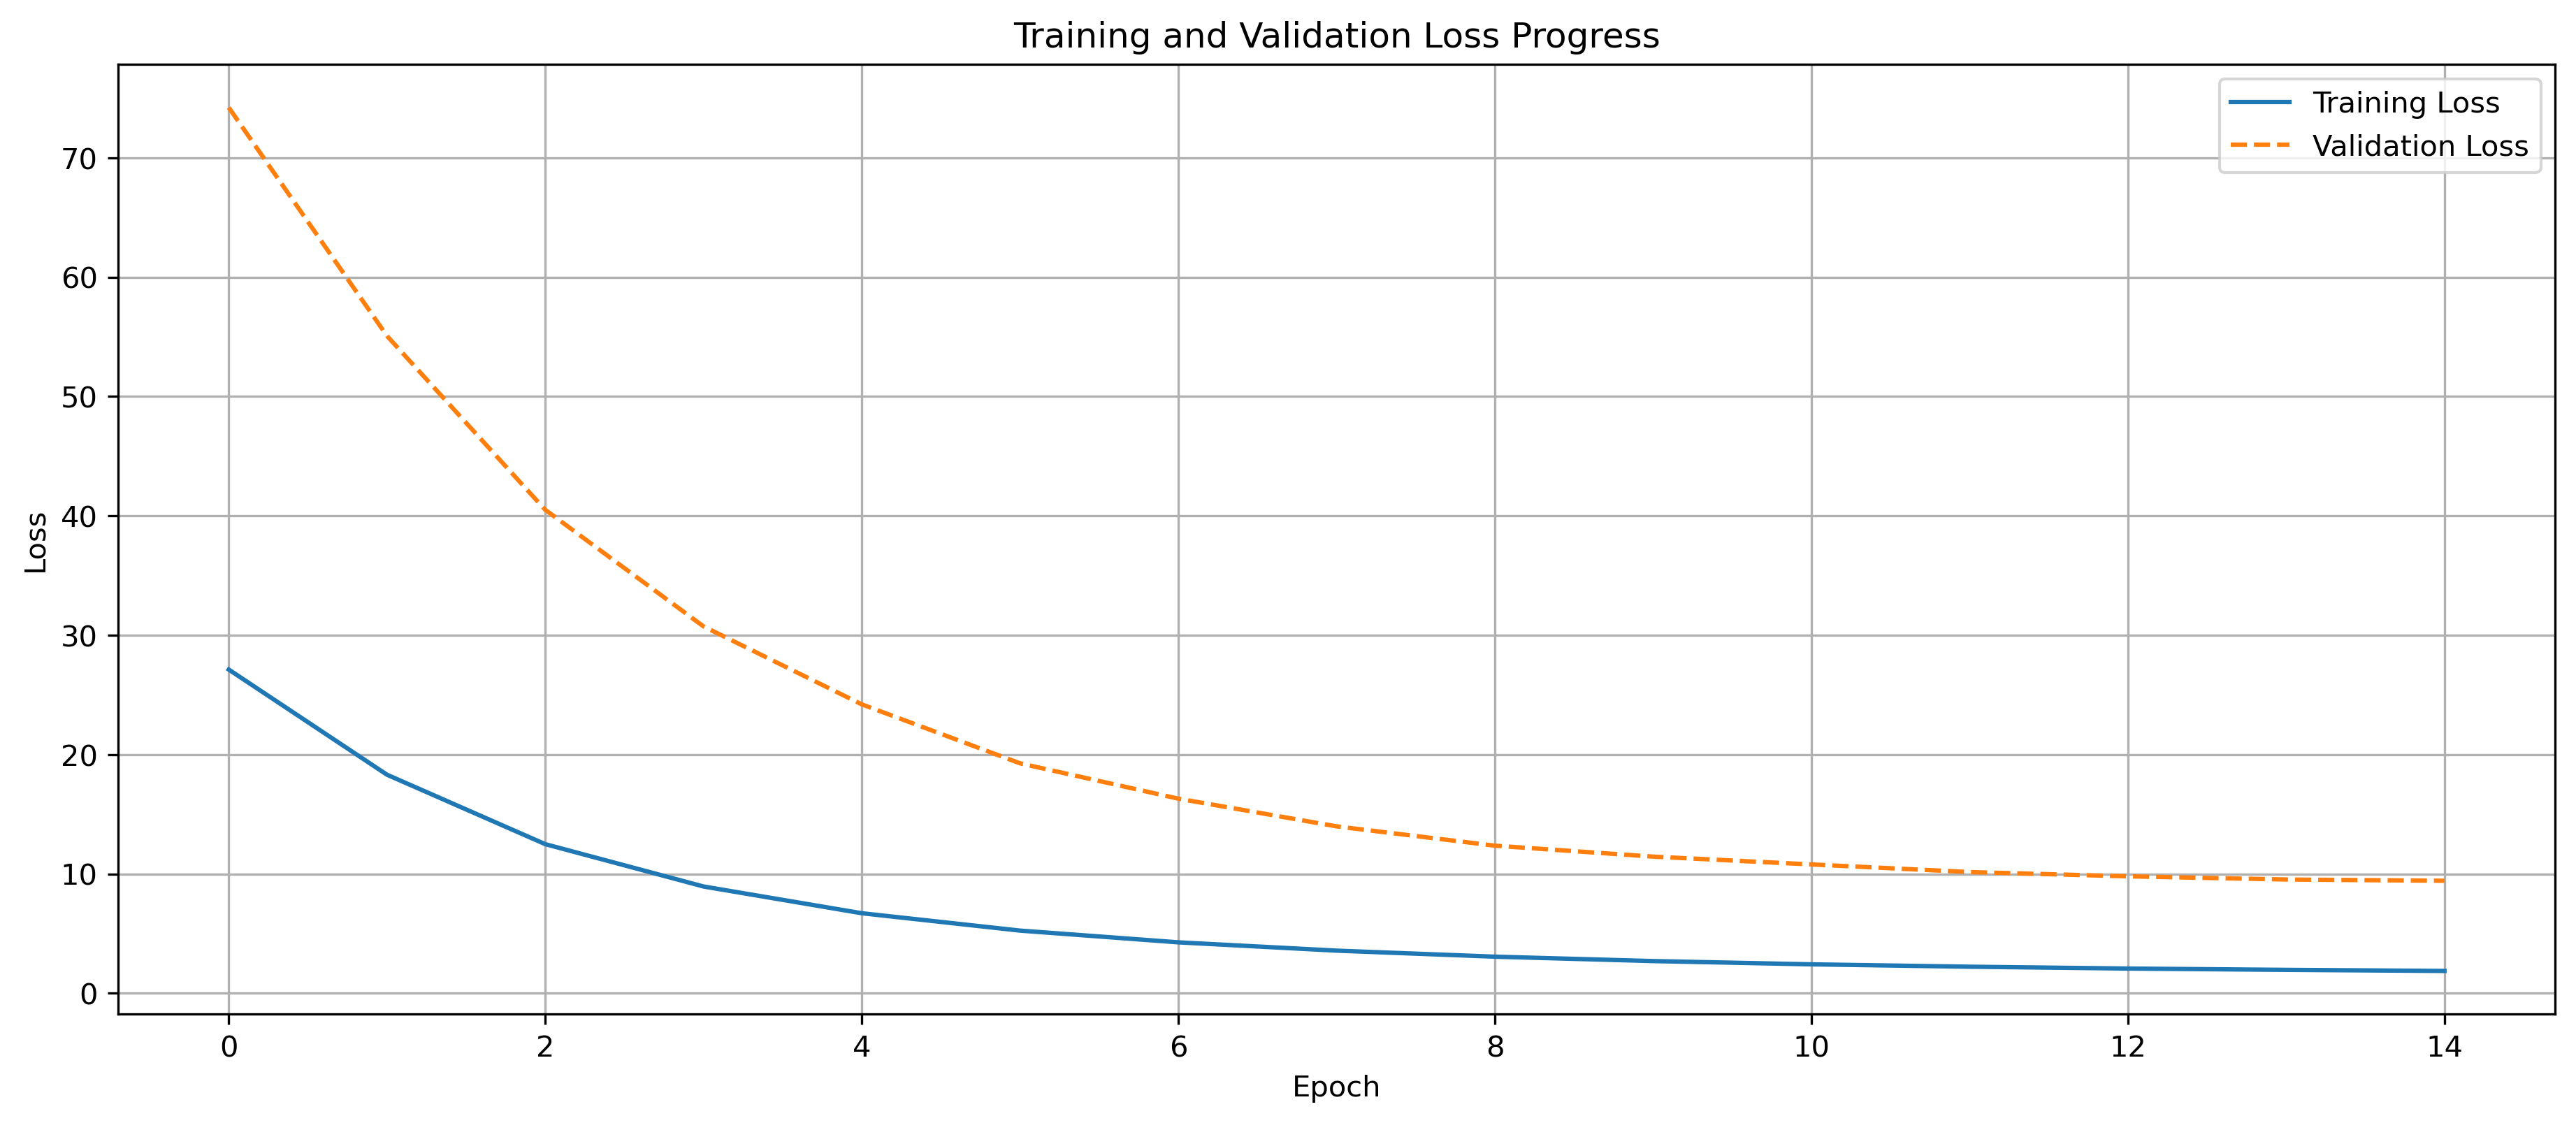
\includegraphics[width=\columnwidth]{../training_validation_loss_Iteration6.png}
    \caption{Training and validation loss for logistic regression (PyTorch)}
    \label{fig:logistic_torch}
\end{figure}

\subsection{Logistic Regression with Scikit-Learn}
Logistic regression implemented using Scikit-Learn offered a computationally efficient alternative. The model was initialized with the saga solver to handle large datasets and incorporated balanced class weights to address class imbalance:

\begin{lstlisting}
lr_model = LogisticRegression(
    penalty="l2",  # Regularization
    C=1.0,         # Regularization strength
    solver="saga"
    max_iter=500,
    random_state=42)
\end{lstlisting}
Normalization was performed using the global mean and standard deviation. The Scikit-Learn implementation yielded the following results:
\begin{center}
    \begin{tabular}{c|c|c|c}
        Accuracy & Precision & Recall & F1 Score \\ 
        \hline 
        0.9023 & 0.1472 &  0.0625 & 0.0885\\
    \end{tabular}
\end{center}
Although the Scikit-Learn implementation performed better than the PyTorch model in terms of F1 score, both approaches struggled with the highly imbalanced data, reaffirming the challenges of this task.

\section{Exploring Lower Percentiles}
Given that all previous attempts to achieve satisfactory performance had failed, the next step was to investigate whether altering the problem definition could yield better results. Specifically, the effect of lowering the percentile threshold used to define "hot" days, as outlined in Section \ref{heatDef}, was examined. For this purpose, the logistic regression model with the "saga" solver, which had previously demonstrated relatively good results, was utilized. Percentile thresholds of 0.5, 0.6, 0.7, 0.8, 0.9, and 0.95 were tested.\\
The results of this investigation are summarized in Table \ref{tab:perc} and visualized in Figure \ref{fig:perc}. It is evident that lowering the percentile threshold simplifies the task, resulting in significantly better performance, as measured by the F1 score. Notably, the F1 score decreases sharply as the percentile threshold approaches 0.95. This indicates that predicting events defined by higher percentiles is substantially more challenging.\\
However, it is important to emphasize that the original objective was to predict heatwaves as defined by the Spanish meteorological service, which corresponds to the 95th percentile. While predictions based on lower percentiles do not directly align with this goal, they can serve as a valuable intermediary step. Models performing well on lower percentiles can inform the selection of suitable architectures, hyperparameter tuning, and data augmentation strategies (e.g., SMOTE). These insights can then be leveraged to optimize models for the more challenging task of predicting heatwaves at the 95th percentile threshold.

\begin{table}[!t]
    \centering
    \caption{Model performance metrics for various percentiles.}
    \label{tab:perc}
    \begin{tabular}{lcccc}
        \toprule
        \textbf{Percentile} & \textbf{Accuracy} & \textbf{Precision} & \textbf{Recall} & \textbf{F1 Score} \\
        \midrule
        50th & 0.7645 & 0.8075 & 0.7965 & 0.8020 \\
        60th & 0.7530 & 0.7804 & 0.7010 & 0.7386 \\
        70th & 0.7452 & 0.7531 & 0.5323 & 0.6238 \\
        80th & 0.7494 & 0.6656 & 0.2781 & 0.3923 \\
        90th & 0.8302 & 0.4024 & 0.0595 & 0.1037 \\
        95th & 0.9164 & 0.1898 & 0.0076 & 0.0147 \\
        \bottomrule
    \end{tabular}
\end{table}

\begin{figure}[!t]
    \centering
    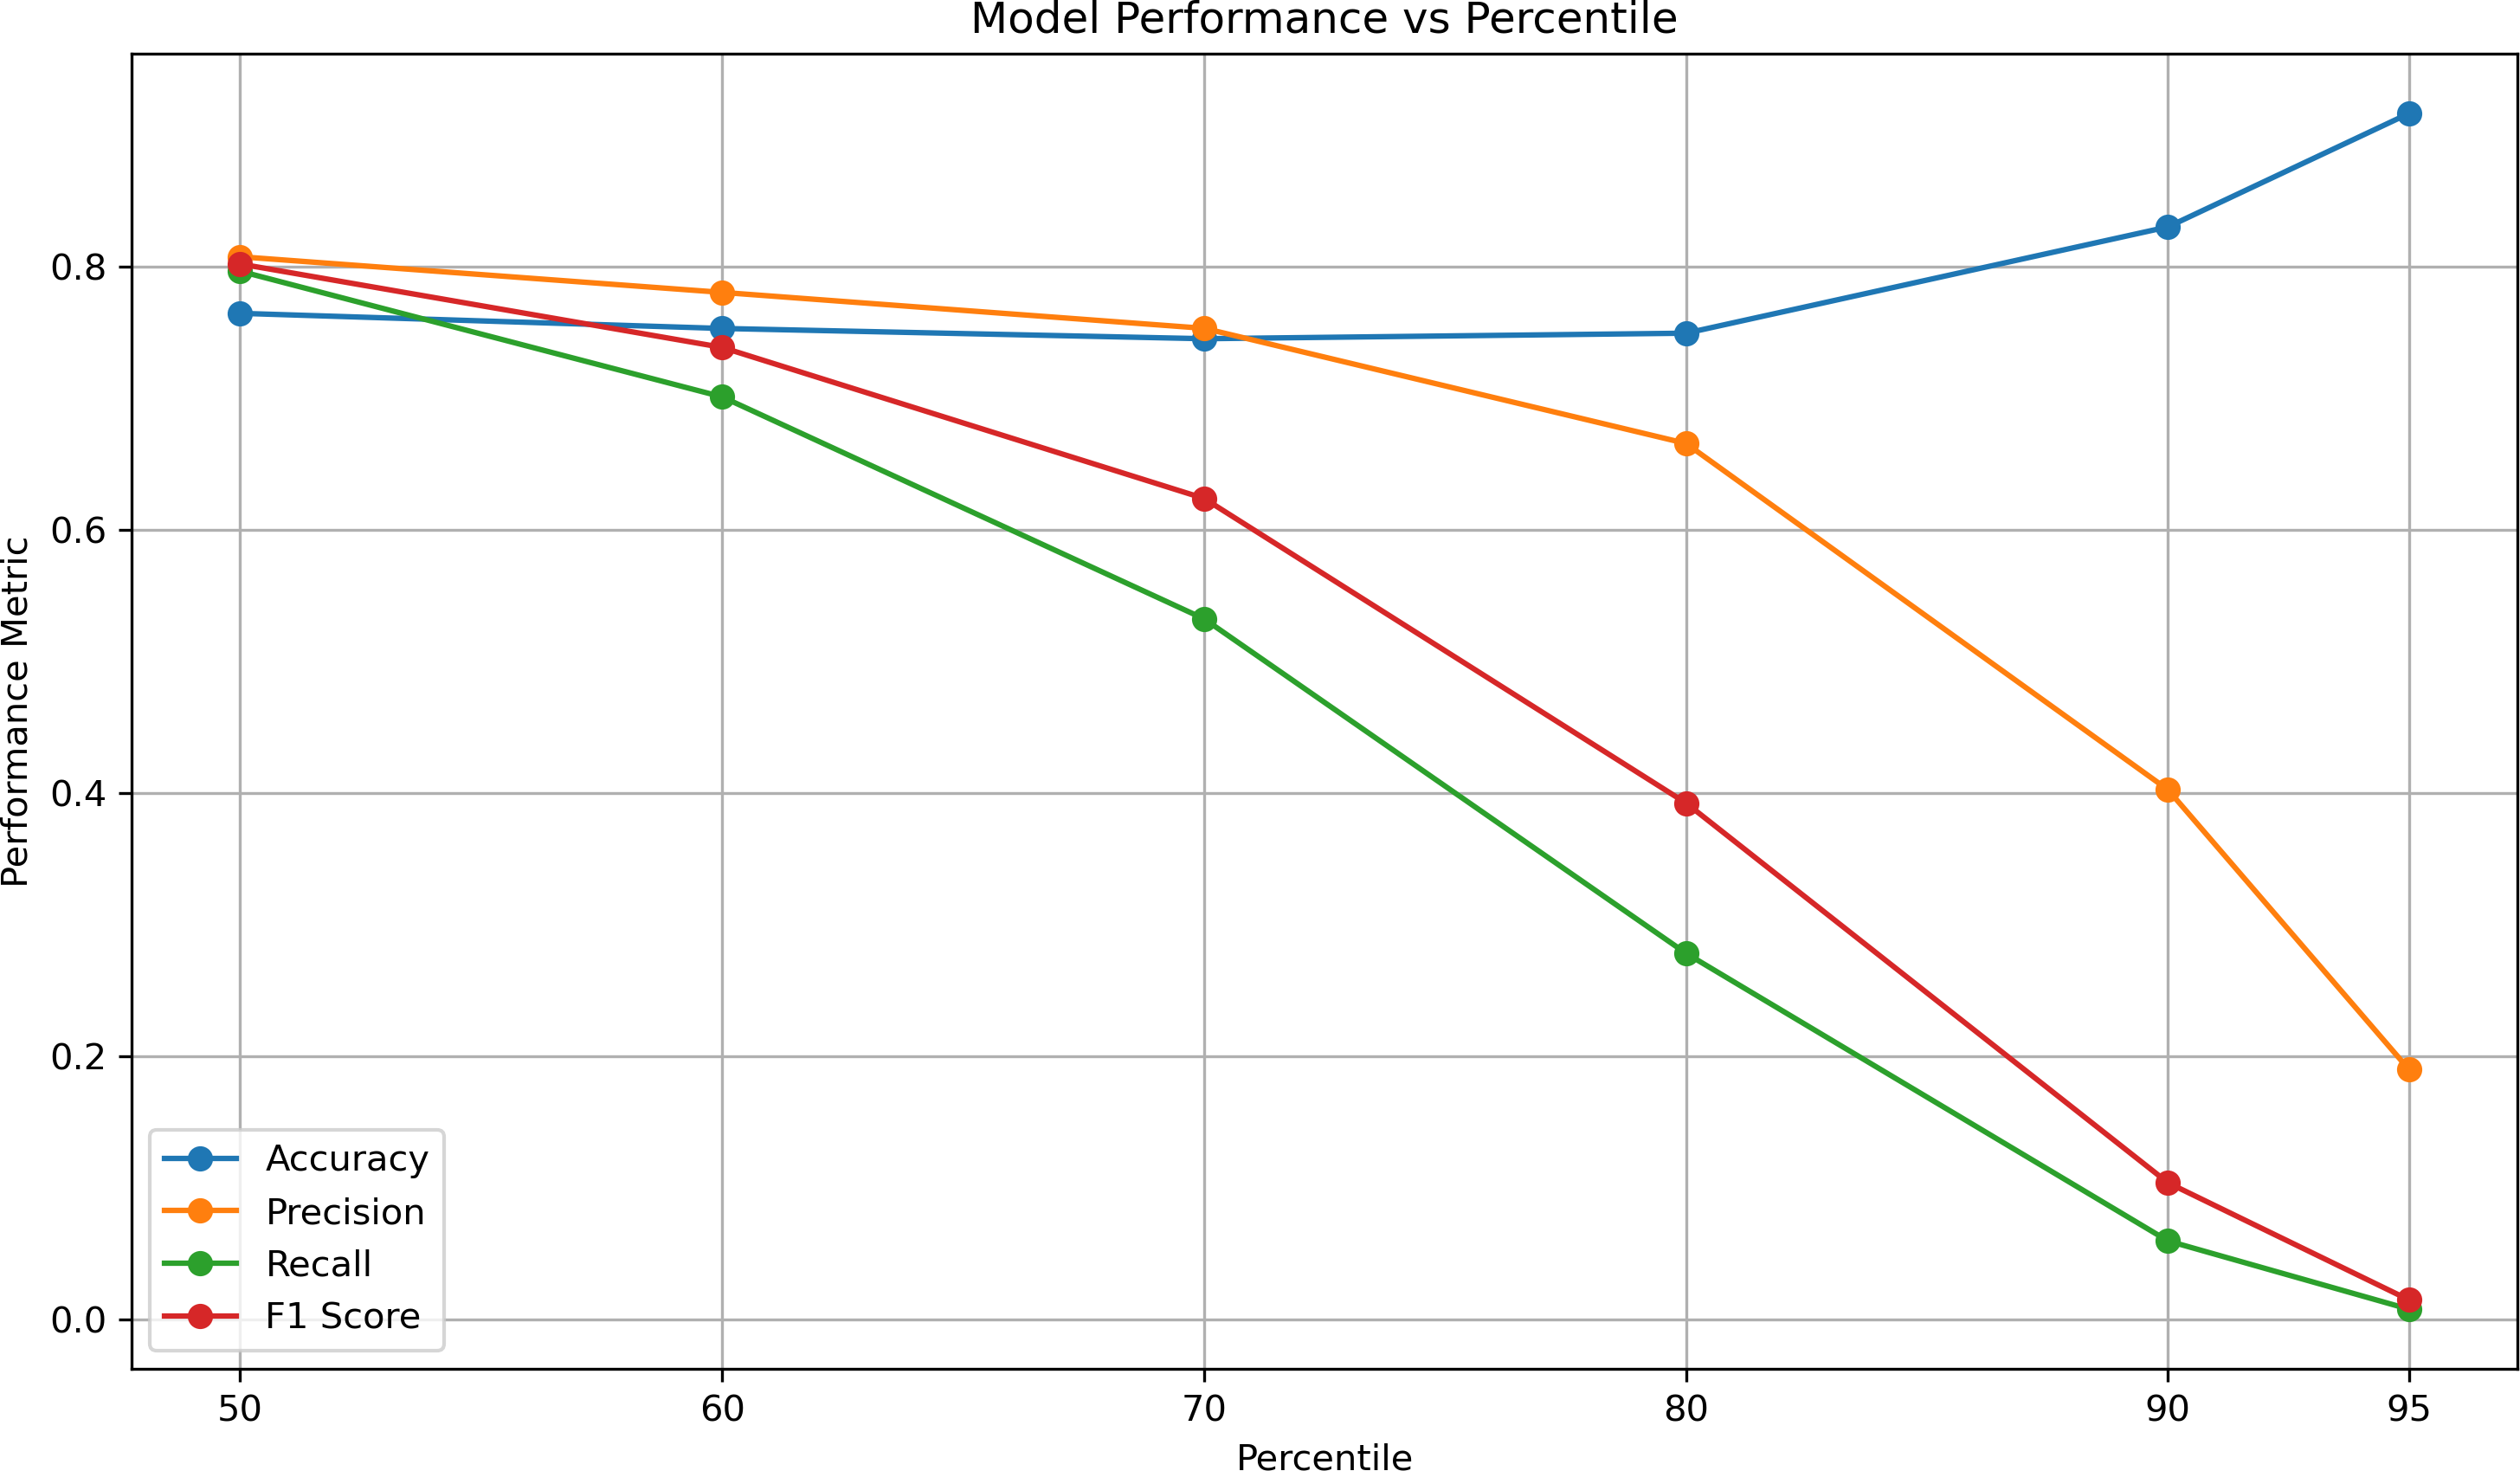
\includegraphics[width=\columnwidth]{./performance_vs_percentile.png}
    \caption{Model performance across different percentiles.}
    \label{fig:perc}
\end{figure}

\section{Different Prediction Timeframes}
To simplify the task for the machine learning model, alternative prediction timeframes were evaluated. Initially, the goal was to predict whether at least 3 of the next 7 days would be "hot." The task was modified to predict whether the next day would be "hot" and then whether at least 2 of the next 3 days would be "hot," using both the 70th and 95th percentiles. \\
The results, shown in Table \ref{tab:timeframe}, highlight that predicting whether the next day is "hot" is significantly easier than the original task for both percentiles. The performance metrics for this simplified task far exceed those of the initial 7-day prediction. Expanding the timeframe to predict whether at least 2 of the next 3 days will be "hot" proves more challenging. For the 95th percentile, the F1 score indicates poor overall performance, though it remains better than the original 7-day prediction task. For the 70th percentile, performance is still acceptable, clearly outperforming the initial task but falling short of the simpler next-day prediction.
\begin{table}[!t]
    \centering
    \caption{Performance metrics for different cases:\\
    \textbf{Case 1}: Predict 1 heat day in 1 day streak;\\
    \textbf{Case 2}: Predict 2 heat days in 3 day streak;\\
    \textbf{Case 3}: Predict 3 heat days in 7 day streak.}
    \label{tab:timeframe}
    \begin{tabular}{lccccc}
        \toprule
        \textbf{Percentile} & \textbf{Case} & \textbf{Accuracy} & \textbf{Precision} & \textbf{Recall} & \textbf{F1 Score} \\
        \midrule
        70th & 1 & 0.9469 & 0.9488 & 0.8836 & 0.9151 \\
        70th & 2 & 0.8530 & 0.8131 & 0.6807 & 0.7411 \\
        70th & 3 & 0.7452 & 0.7531 & 0.5323 & 0.6238 \\
        95th & 1 & 0.9431 & 0.9317 & 0.3436 & 0.5020 \\
        95th & 2 & 0.9346 & 0.6541 & 0.0648 & 0.1179 \\
        95th & 3 & 0.9164 & 0.1898 & 0.0076 & 0.0147 \\
        \bottomrule
    \end{tabular}
\end{table}


\section{Possible Future Work}
After an in-depth examination, it can be concluded that achieving high performance for the initial task within the current framework is highly unlikely. As demonstrated in the previous sections, simplifying the problem either in the temporal domain or by relaxing the criteria for defining "hot" days leads to significant performance improvements, with results that are highly satisfactory. However, if the objective remains to tackle the original, more complex problem, the current framework must undergo fundamental changes.\\
A promising direction would be to incorporate weather data from adjacent locations in addition to the target location. This approach aligns with standard practices in weather forecasting, as weather patterns are highly dependent on regional interactions. However, implementing this strategy would require more complex data preprocessing and significantly higher computational resources. Even with the current preprocessing framework, a laptop with 16GB of memory struggles to handle the workload, making it necessary to migrate the project to a cloud-based service such as Google Colab. While attempts to use such platforms were made earlier, unresolved errors and compatibility issues hindered progress.\\
Another critical step would be to conduct a thorough review of relevant literature and research on similar projects. Adopting methods and techniques that have already demonstrated success in related studies could provide valuable insights and potentially steer the project in a more promising direction. Ideally, this review should have been conducted earlier in the project, as it might have prevented efforts from being directed toward less fruitful approaches.\\
By addressing these considerations, the project could be significantly improved, whether by simplifying the problem further or by fundamentally redesigning the framework to tackle the original task more effectively.


\section{Allocation of tasks}
\begin{itemize}
\item Setting up git: Jonas
\item Generating Dataset: Jonas
\item Data Preprocessing: Jonas
\item Machine Learning, optimizing Neural Network: Both
\item SMOTE: Both
\item Anomaly detection: Ana
\item Investigating effect of using different percentile: Jonas
\item Writing Report: Both
\end{itemize}
For more information the commit history can be consulted (\href{https://github.com/JonasThalmeier/MALIS_heatForecast}{GitHub Repository})
\section{Usage of Artificial Intelligence}
Artificial Intelligence, specifically ChatGPT, was employed in various aspects of the project to enhance efficiency and streamline processes.

\begin{itemize}
\item \textbf{Code Generation:} ChatGPT was utilized to generate lines and blocks of code based on the explicit design choices made regarding data preprocessing, structuring, and the selection of models and networks. This significantly accelerated the initial setup of the data pipeline, enabling the first model to be trained and tested without errors. Additionally, since Jonas, who handled the data preprocessing, was not entirely familiar with the variety of techniques for restructuring data to facilitate efficient machine learning, ChatGPT was instrumental in identifying and implementing the most effective methods.

\item \textbf{Debugging:} When the code crashed or exhibited unexpected behavior, ChatGPT played a crucial role in diagnosing and resolving the issues. This proved particularly helpful in addressing errors that required a deeper understanding of specific tools or libraries.

\item \textbf{Text Refinement:} As non-native English speakers, the team leveraged ChatGPT's capabilities to refine the phrasing of text in the report. This ensured that the final document was clear, professional, and easy to read, enhancing its overall quality and accessibility.
\end{itemize}

\end{document}
